\section{Wohlstand}
\subsection{Die volkswirtschaftliche Diskussion}
Dies sind die wirtschaftlichen Ziele eines Landes:
\begin{itemize}
	\item Hoher Wohlstand
	\item Tiefe Arbeitslosigkeit
	\item Stabile Preise und Wechselkurse
	\item Nachhaltige Staatsfinanzierung
	\item Stabiles Finanzsystem
\end{itemize}
Der Weg dazu führt entweder über Markt oder Staat.

\subsection{Mikro-/Makroökonomie}
\begin{multicols}{2}
\subsubsection{Mikroökonomie}
Teilgebiet der Volkswirtschaftslehre, das sich mit den Entscheidungen der Haushalte und der Unternehmen sowie mit deren Zusammenspiel auf einzelnen Märkten befasst.
\columnbreak
\subsubsection{Makroökonomie}
Teilgebiet der Volkswirtschaftslehre, das sich mit gesamtwirtschaftlichen Phänomenen wie Inflation, Konjunkturschwankungen oder langfristigem Wachstum befasst.
\end{multicols}

\subsection{Makroökonomisches Grundmodell}
\begin{multicols}{2}
\subsubsection{Aggregierte Nachfrage $AN$}
Stellt die gesamtwirtschaftliche Nachfrage nach Gütern (Waren und Dienstleistungen) in Abhängigkeit vom Preisniveau dar. Die aggregierte Nachfragekurve wird auch gesamtwirtschaftliche Nachfragekurve genannt.
Die vier volkswirtschaftlichen Akteure und ihre Nachfrage:
\begin{itemize}
	\item Haushalt $\rightarrow$ Konsum
	\item Unternehmen $\rightarrow$ Investitionen
	\item Staat $\rightarrow$ Staatsausgaben
	\item Ausland $\rightarrow$ Nettoexporte = Exporte - Importe	
\end{itemize}
\columnbreak
\subsubsection{Aggregierte Angebotskurve $AA$}
Stellt das gesamtwirtschaftliche Angebot in Abhängigkeit vom Preis dar. Die aggregierte Angebotskurve wird auch gesamtwirtschaftliche Angebotskurve genannt.
\end{multicols}

\begin{multicols}{2}
\subsubsection{langfristig aggregiertes Angebot $AA_L$}
Die aggregierte Angebotskurve in der langen Frist (AA\textsubscript{L}) orientiert sich an den Produktionsmöglichkeiten einer Volkswirtschaft. Real ändert sich nichts, wenn sich alle Preise gleichermassen verändern. Somit verläuft die AA-Kurve in der langen Frist vertikal, die Kapazitätsgrenze ist also unabhängig vom Preisniveau.\\
Produktionsfaktoren:
\begin{itemize}
	\item Arbeit
	\item Kapital
	\item Technologie
	\item Boden und Ressourcen
\end{itemize}
Je tiefer das Preisniveau, desto höher die Nachfrage.
\columnbreak
\subsubsection{kurzfristig aggregiertes Angebot $AA_K$}
Aufgrund der unterschiedlichen Flexibilität der Preise in der kurzen Frist (gewisse Preise passen sich schneller an als andere) beobachtet man eine positive Steigung der kurzfristigen aggregierten Angebotskurve AA\textsubscript{K}. An der Kapazitätsgrenze sind die Produktionsfaktoren optimal, nicht aber maximal ausgelastet. Durch Überstunden und maximale Auslastung der Infrastruktur kann die $AA_K$-Kurve über der Kapazitätsgrenze liegen.
\end{multicols}
\clearpage

\begin{multicols}{2}
\subsubsection{Makroökonomisches Gleichgewicht}
Das Makroökonomische Gleichgewicht (= ausgelastete Wirtschaft) ist erreicht, wenn sich die Kurven $AN$ und $AA_K$ bei der Kapazitätsgrenze schneiden. 
\begin{description}
	\itemsep-0.5em
	\item [Preisniveau:] wird mit einem definierten Güterkorb berechnet, z.B. dem Landesindex der Konsumentenpreise oder dem zeitlich vorauslaufenden Produzentenpreisindex
	\item [reales BIP:] gesamte, zu konstanten Preisen bewertete Produktion von Gütern und Dienstleistungen (inflationsbereinigte Wertschöpfung)
	\item [Kapazitätsgrenze:] reales BIP das mit der bestehenden Ausstattung an Produktionsfaktoren bei Normalauslastung produziert werden kann (auch \textit{potenzieller Output} genannt)
\end{description}
\columnbreak
Langfristig kehrt die Wirtschaft zu einer normalen Auslastung der Kapazitäten zurück, d.h. in ein gleichgewichtiges BIP, das unabhängig von der aggregierten Nachfrage ist.
%\columnbreak
\includegraphics[width=1\linewidth]{images/makro.png}
\end{multicols}

\begin{multicols}{2}
\subsection{Bruttoinlandprodukt (BIP)}
Das BIP gibt den Gesamtwert aller Güter (Produkte und Dienstleistungen), welche innerhalb eines Jahres innerhalb der Grenzen der Volkswirtschaft hergestellt wurden abzüglich der notwendigen Vorleistungen (im laufenden Jahr).\\
Der Anteil des Staatskonsums am BIP nennt man Staatsquote. Dia Nachfrage des Auslands fliesst in Form von Nettoexporten (Exporte minus Importe) in das BIP ein.

\subsubsection{Reales/Nominales BIP}
\begin{itemize}
	\item Das nominale BIP gibt die Wertschöpfung zu Marktpreisen an.
	\item Das reale BIP gibt die \textbf{Wertschöpfung} (=BIP) inflationsbereinigt (zu konstanten Preisen) an.
	\item Das reale BIP der Schweiz beträgt \textbf{ca. 658 Mia.} (2016p) Franken. Die letzte verfügbare definitive BIP-Kennzahl des BFS ist aus dem Jahr 2014.
\end{itemize}
\vfill\null
\columnbreak
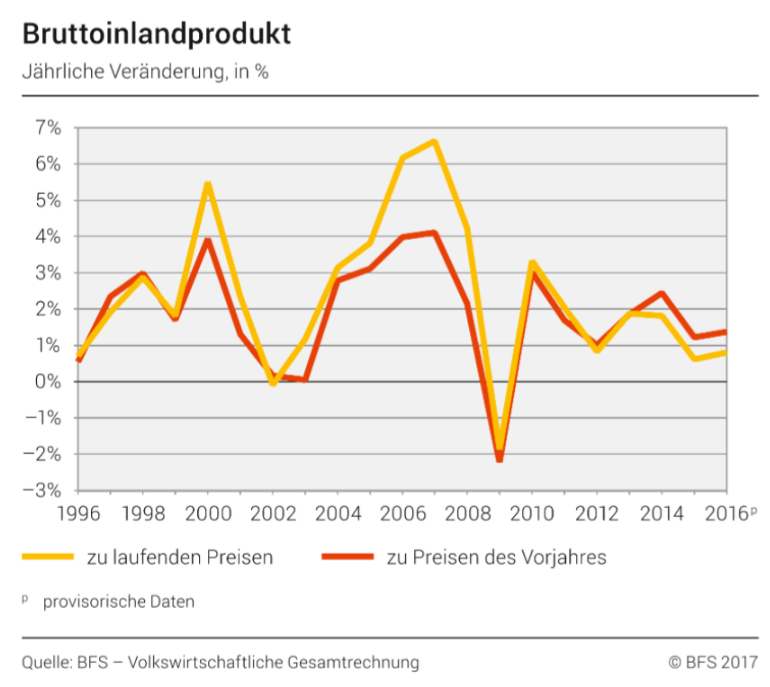
\includegraphics[width=\linewidth]{images/realbip.png}	
\end{multicols}

\begin{multicols}{2}
\subsubsection{Zusammenhang BIP \& Wohlstand}
Je höher das BIP, desto höher ist die Lebensqualität und der soziale Fortschritt eines Landes. Es ist aber zu erwähnen, dass für die Lebensqualität auch Umstände wie Umwelt, Kriminalität, Wohnsituation, Einkommen, Arbeitsplätze, Gesundheit und Bildung eine Rolle spielen. Bei armen Ländern führt ein geringes Wachstum zu spürbarem Anstieg der Lebensqualität. Um das BIP zu analysieren gibt es drei Ansätze:
\begin{description}
	\itemsep-0.5em
	\item [Produktionsansatz:] Wertschöpfung der Wirtschaftsakteure
	\item [Einkommensansatz:] Bezahlung der Produktionsfaktoren (= Arbeit, Technologie)
	\item [Verwendungsansatz:] Verwendung des Einkommens der Wirtschaftssubjekte
\end{description}
\vfill\null
\columnbreak
\includegraphics[width=\linewidth]{images/bip.png}\\
Angebot (Produktion) $\rightarrow$ $AA_K$\\
Nachfrage (Verwendung) $\rightarrow$ AN
\end{multicols}


\begin{multicols}{2}
	\subsubsection{Bruttonationaleinkommen (BNE)}
	Das BNE (früher Bruttosozialprodukt) wird aufgrund der erbrachten Leistungen der Staatsangehörigen \textbf{unabhängig der Grenzen} errechnet.
	\columnbreak
	\subsubsection{Aufteilung des BIP in der Schweiz}
	1/6 $\rightarrow$ Arbeitgeber\\
	4/6 $\rightarrow$ Arbeitnehmer (=Lohnquote)\\
	1/6 $\rightarrow$ Abschreibungen
\end{multicols}

\subsubsection{72er Regel}
Die Zeit (x), in der sich eine Kapitaleinlage mit Zinssatz p (in \%) verdoppelt.
\begin{equation*}
	x=\frac{72}{p} \quad \frac{72}{4\%}= 18 Jahre
\end{equation*}

\clearpage
\pagebreak